\documentclass[10pt]{article}
\usepackage[english]{babel}
\usepackage{hyperref}
\usepackage[utf8]{inputenc}
\usepackage[T1]{fontenc}
\usepackage{amsmath,amsfonts,amssymb,amsthm,cancel,siunitx,
calculator,calc,mathtools,empheq,latexsym}
\usepackage{subfig,epsfig,tikz,float}
\usepackage{booktabs,multicol,multirow,tabularx,array}
\usepackage[square,sort,comma,numbers]{natbib}
\usepackage{graphicx}
\graphicspath{ {./images/} }
\setlength{\parindent}{0pt}
\setlength{\parskip}{5pt}
\textwidth 13.5cm
\textheight 19.5cm
\columnsep .5cm
\title{\renewcommand{\baselinestretch}{1.17}\normalsize\bf%
\uppercase{
	Studiul tehnicilor de recunoastere \\
	si clasificare a imaginilor 2D}
}
\author{
Barbu Vlad Alexandru
}

\begin{document}

\date{}

\maketitle

\vspace{-0.5cm}

\begin{center}
{\footnotesize 
Facultatea de Matematica si Informatica, \\
Universitatea din Bucuresti, \\
Bucuresti, Romania \\
vlad.barbu@s.unibuc.ro \\
}
\end{center}

% -------------------------------------------------------------------
% Abstract
\bigskip
\noindent
{\small{\bf ABSTRACT.}
		Automatizarea clasificarii imaginilor si recunoasterea predictibila 
	a formelor de interes din contextul acestora reprezinta o problema complexa,
	avand implicatii majore in multe domenii stiintifice. Definirea unui
	proces sistematic de prelucrare, identificare si clasificare reprezinta
	un demers necesar abordarii acestei probleme. Acest raport incearca sa
	ofere o viziune de ansamblu asupra solutiilor existente, 
	avand drept obiect de studiu pentru analiza si implementarea acestora - recunoasterea 
	si extragerea informatiei din cadrul unui document scos la imprimanta (deseori pornind
	de la structura unui tipizat de baza, fiind completat ulterior in format digital
	sau cu scris de mana).
}

\medskip
\noindent
{\small{\bf Cuvinte cheie}{:} Recunoasterea formelor. Prelucrarea imaginilor. Clasificarea imaginilor 2D.
}

\baselineskip=\normalbaselineskip
% -------------------------------------------------------------------

\section{Introducere}\label{sec:1}

\> {\bf Procesul de recunoastere a formelor} poate fi vazut drept o inlantuire de proceduri cu ajutorul
carora se poate ajunge la un rezultat concludent de clasificare a unui obiect de
interes din cadrul unei multimi de entitati observabile. O astfel de metoda de recunoastere
devine utila mai ales atunci cand abordarea directa este imposibila - atunci cand o 
clasificare manuala nu este fezabila (in cazul in care nevoia de recunoastere este una recurenta).

\> {\bf Descrierea unui proces robust de clasificare automata a imaginilor} consta in
stabilirea unui set de reguli in baza caruia, datele de intrare pot fi grupate in clase
identificabile. O clasa identificabila este reprezentata de o multime finita de factori
cantitativi si calitativi cu ajutorul carora unui obiect observabil ii este asociat un numar de
atribute semnificative - contextul de identificare a unei astfel de clase este determinat de o colectie
predefinita de metadate. Metoda folosita pentru delimitarea claselor identificabile reprezinta un
caz particular specific domeniului de interes al aplicatiei concrete. 

\newpage

\section{Descrierea unui sistem de recunoastere}\label{sec:2}

\> Un sistem robust si eficient de recunoastere a formelor va oferi rezultate corecte, predictibile
urmand o inlantuire de proceduri de transformare, prelucrare, extractie si clasificare.
Componentele principale ale unui sistem de recunoastere si clasificare a formelor sunt urmatoarele:

\begin{itemize}
    \item {\bf Componenta de preprocesare} - cu ajutorul acestei componente se vor normaliza datele de intrare
	(mediul de provenienta al acestora fiind necunoscut, stabilirea unui standard este necesara)
	si se vor evidentia obiectele de interes prin eliminarea impuritatilor
	\item {\bf Selectorul de obiecte de interes} - in cadrul acestei etape, imaginea va fi parcursa
	si redusa la o multime de entitati de interes (structura observabilelor va fi definita
	prin intermediul acestei componente, urmand ca aceasta sa fie definitia standardului de metadate
	folosit de-a lungul procesului de recunoastere)
    \item {\bf Selectorul de atribute semnificative} - cu ajutorul acestuia, vom putea identifica
    factorii cantitativi si calitativi pe care un anumit observabil ii respecta (acesti factori trebuie sa fie predefiniti
	cu ajutorul unor descriptori relevanti domeniului de interes al aplicatiei)
    \item {\bf Componenta de masurare a atributelor} - responsabilitatea acestei componente este aceea de
    a calcula "importanta" atributelor asociate fiecarui observabil prin invocarea unui set
	predefinit de metrici si metode discriminative relevante pentru fiecare context de identificare, urmata
	de agregarea rezultatelor obtinute
    \item {\bf Clasificatorul} - etapa finala a procesului de recunoastere este reprezentata de
    efectuarea unei alegeri prin compararea masuratorilor efectuate in pasii anteriori pentru fiecare clasa
	identificabila predefinita
\end{itemize}

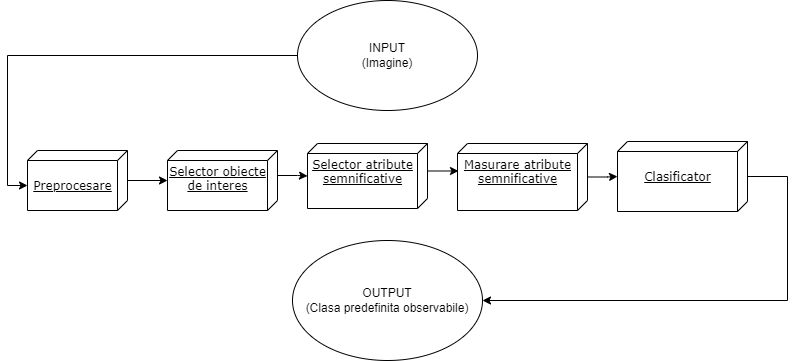
\includegraphics[scale=0.5]{componente}


\newpage

\section{Reprezentarea imaginilor}\label{sec:3}

\> Din punct de vedere matematic, o imagine poate fi reprezentata sub forma unei
functii de doua variabile:

\begin{itemize}
	\item In cazul imaginilor formate doar din tonuri de gri (i.e. Grayscale),
	valorile functiei reprezinta luminanta pixelilor
	
	\begin{equation}\label{eq:1}
		f(x,y) : R^2 -> R
	\end{equation}

	\item In cazul imaginilor color, valorile reprezinta un vector de 3 elemente,
componente ale spatiului de culori ales (un exemplu ar fi spatiul de culori RGB:
unde R - red, G - green, B - blue)

	\begin{equation}\label{eq:2}
		f(x,y) : R^2 -> R^3
	\end{equation}

\end{itemize}

\> Inainte de a putea prelucra o imagine, aceasta va trebui discretizata din punct
de vedere spatial. Procesul aferent discretizarii spatiale a
coordonatelor (i.e. {\it esantionare}), descrie un mod de aproximare a unei imagini continue
de tipul f(x,y), cu o matrice 2-dimensionala de tipul MxN, unde M reprezinta numarul de randuri,
iar N reprezinta numarul de coloane de pixeli.

\begin{equation}\label{eq:3}
	f(x,y) = p_{x,y}
\end{equation}

\[
\begin{bmatrix}
    p_{0,0}       & p_{0,1} & p_{0,2} & \dots & p_{0,m-1} \\
    p_{1,0}       & p_{1,1} & p_{2,2} & \dots & p_{1,m-1} \\
    \hdotsfor{5} \\
    p_{n-1,0}       & p_{n-1,1} & p_{n-1,2} & \dots & p_{n-1,m-1}
\end{bmatrix}
\]

\> Trebuie sa tinem cont de faptul ca discretizarea unei imagini este un proces insotit de zgomot - {\it eroare de cuantizare}.
Una dintre cele mai folosite metode de cuantizare este cuantizarea uniforma - intervalele
functiei de cuantizare sunt egale. \\

\> {\bf O imagine digitala} este reprezentata de o structura de date bidimensionala, unde un
element (x, y) al acesteia poarta numele de pixel.

\newpage

\section{Preprocesarea imaginii si eliminarea zgomotului}

\> Zgomotul de imagine este o variație aleatorie a luminozității sau a informațiilor de culoare
din imagini și este, de obicei, un aspect al zgomotului electronic.
Acesta reprezinta un produs secundar nedorit al captării imaginii, care ascunde informațiile dorite.

\> Sensul original al cuvântului "zgomot" era "semnal nedorit". Prin analogie, fluctuațiile electrice nedorite sunt, de asemenea, numite "zgomot".

\> Zgomotul de imagine poate varia de la pete aproape imperceptibile pe o fotografie digitală făcută în condiții de lumină bună,
până la imagini care sunt aproape în întregime zgomot,
din care se poate obține o cantitate mică de informații chiar si prin metode de procesare sofisticată.
Un astfel de nivel de zgomot ar fi inacceptabil într-o fotografie, deoarece ar fi imposibil să se determine subiectul.

\begin{center}

  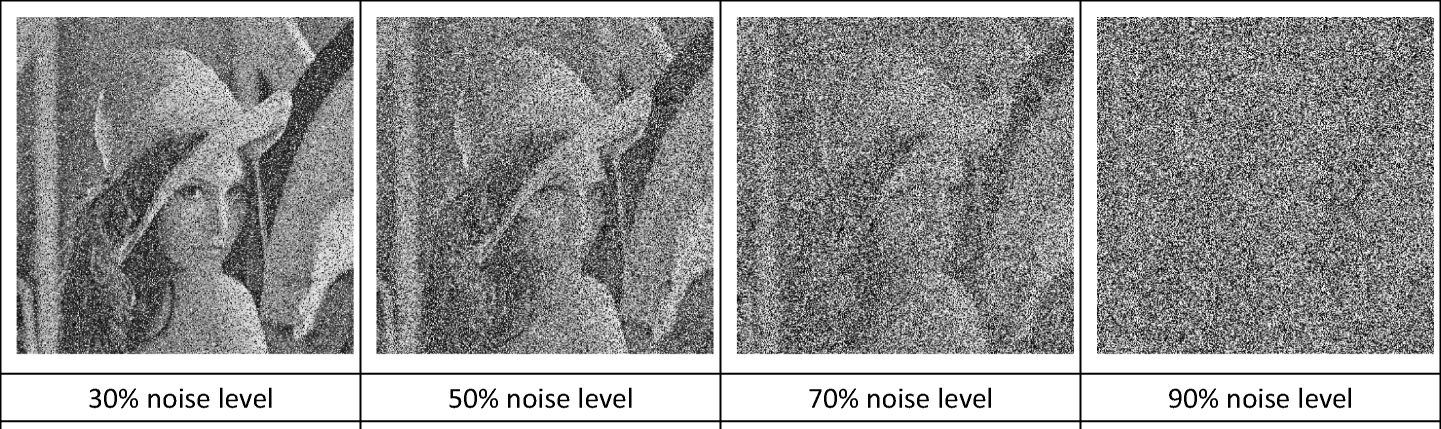
\includegraphics[scale=0.2]{noisy-images}
  
\end{center}

\> Procesele de eliminare a zgomotului din cadrul unei imagini sunt cunoscute si sub numele de
operatii de filtrare. Scopul acestora este reprezentat de nevoia evidentierii muchiilor si reliefarea entitatilor observabile.

\> Trei dintre cele mai folosite metode de filtrare sunt:


\begin{itemize}

	\item Filtrul trece-jos - procedura de filtrare a zgomotului realizat prin operatii de uniformizare a spectrului imaginii
	\item Filtrul trece-banda - procedura comuna de eliminare a zgomotului in domeniile in care se prelucreaza imagini obtinute prin metode de teledetectie
	\item Filtrul trece-sus - procedura utilizata in cazul in care evidentierea contururilor este principala nevoie de prelucrare

\end{itemize}

\> De asemenea, metodele de filtrare si analiza a semnalelor unidimensionale pot fi extinse cu usurinta in mediul semnalelor bidimensionale - putem
descompune un semnal bidimensional in sume de semnale sinusoidale.

\newpage

\> Tehnicile de filtrare sunt utilizate pentru a îmbunătăți și modifica imaginile digitale.
De asemenea, filtrele de imagine sunt utilizate pentru a reduce neclaritatea și zgomotul, pentru a îmbunătăți claritatea
și pentru a detecta marginile.

\> Filtrele de imagine sunt utilizate în principiu pentru suprimarea frecvențelor înalte
(tehnici de netezire) și joase (îmbunătățirea imaginii, detectarea marginilor).

\begin{center}

  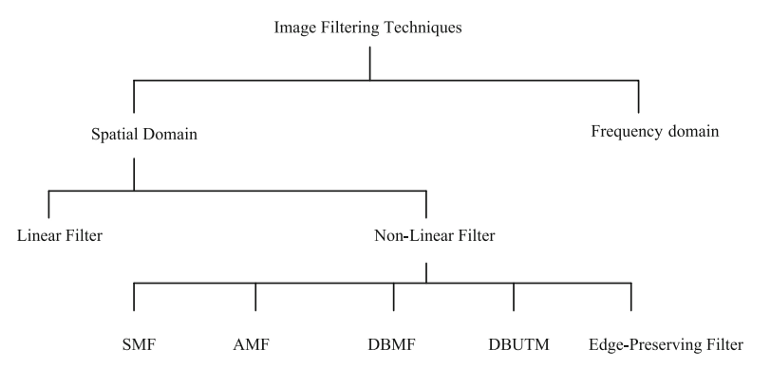
\includegraphics[scale=0.5]{image-filters-classification}
  
\end{center}

\> În conformitate cu această clasificare, filtrele de imagine pot fi împărțite în două categorii principale:

\begin{itemize}

	\item Filtrarea spațială - metoda tradițională de filtrare a imaginilor, care se utilizează direct pe pixelii imaginii
	\item Filtrele în domeniul frecvenței - metoda utilizata pentru a elimina frecvențele înalte și joase și pentru netezire
	
\end{itemize}

\> Filtrele neliniare sunt utilizate pentru a detecta marginile. Aceste tehnici de filtrare sunt mai eficiente decât filtrele liniare.
În cazul filtrării liniare, detaliile și marginile imaginii tind să se estompeze.

\> Filtrul Gaussian, filtrul Laplacian și filtrul de medie de vecinătate (medie) pot fi identificate ca exemple de filtre liniare.
Filtrele mediane sunt filtre neliniare.

\newpage

\subsection{Filtrul median}

\> Filtrul median este un filtru neliniar care înlocuiește valorile fiecărui pixel cu valorile mediane ale pixelilor săi vecini.


\> Acesta este un mod eficient de a elimina zgomotul de tip "salt and pepper" - o formă de zgomot, cunoscuta și sub numele de 
zgomot de impuls, poate fi cauzat de perturbații bruște în semnalul de imagine si se prezintă sub forma unor pixeli albi și negri cu apariție dispersată.

\begin{center}

  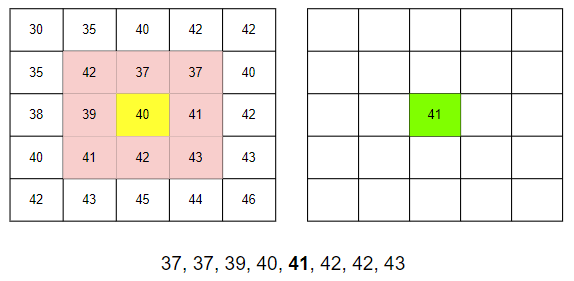
\includegraphics[scale=0.5]{filtru-median-masca}
  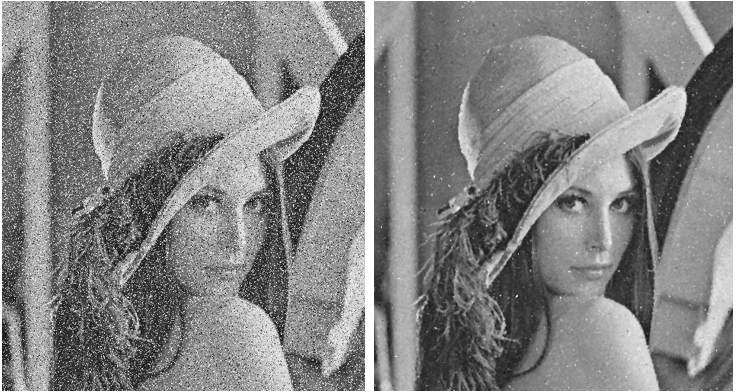
\includegraphics[scale=0.5]{filtru-median}

\end{center}

\newpage

\subsection{Filtrul Laplacian}

\> Tehnica de netezire Laplace este utilizată în principal pentru a detecta marginile imaginii.
Aceasta evidențiază discontinuitățile nivelului de gri. Se bazează pe a doua derivare spațială a unei imagini.

\> Pentru a defini operatorul Laplacian, a fost utilizată ecuația de mai jos:

\begin{center}

  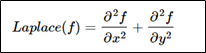
\includegraphics[scale=0.5]{filtru-laplacian-ecuatie}

\end{center}

\> Detectorul de margini Laplace utilizează un singur nucleu.
Pentru a detecta marginile unei imagini, acest nucleu detectează derivatele de ordinul 2 ale nivelurilor de
intensitate ale imaginii, utilizând o singură trecere.

\> Putem utiliza cel de-al doilea nucleu din imaginile de mai jos pentru a detecta marginile cu diagonale.
Acesta va oferi o aproximare mai bună. De asemenea, metoda Laplace oferă calcule mai rapide decât celelalte.

\begin{center}

  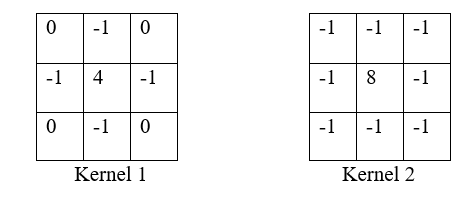
\includegraphics[scale=0.5]{filtru-laplacian-masca}
  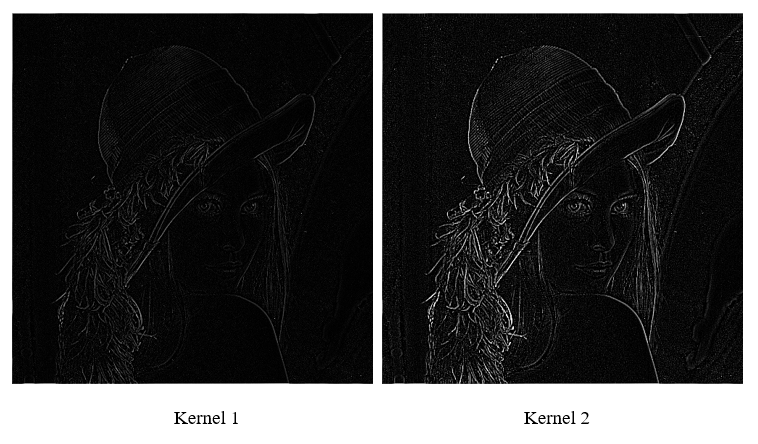
\includegraphics[scale=0.5]{filtru-laplacian}

\end{center}

\newpage


\subsection{Filtrul Gaussian}

\> Acest filtru este un operator convoluțional 2-D. Se utilizează pentru a estompa imaginile.
De asemenea, elimină detaliile și zgomotele. Filtrul gaussian este similar cu filtrul mediu,
dar principala diferență este că filtrul gaussian utilizează un nucleu. Acest nucleu are forma unei "cocoașe" gaussiene.

\> Nucleul gaussian ponderează pixelii din centrul său mult mai puternic decât cei de la limitele sale.
Există diferite nuclee gaussiene. În funcție de dimensiunea nucleului, imaginea de ieșire va fi diferită.

\begin{center}

  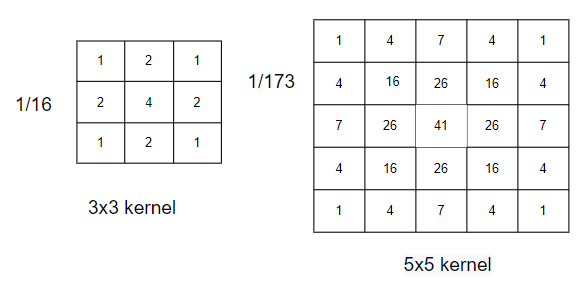
\includegraphics[scale=0.5]{filtru-gaussian-masca}
  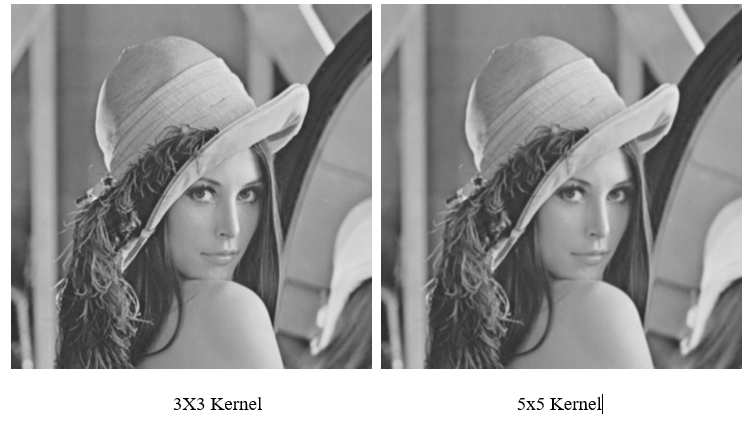
\includegraphics[scale=0.5]{filtru-gaussian}

\end{center}


\section{Segmentarea imaginii}

\> Segmentarea imaginilor este procesul prin care o imagine digitală este împărțită în diferite subgrupuri (de pixeli)
numite entitati observabile, reducand complexitatea imaginii, astfel analiza acesteia devenind mai simplă.

\> Procesele de acest tip utilizeaza diverși algoritmi de segmentare a imaginilor pentru a diviza și grupa un anumit set de pixeli din imagine.
În acest fel, atribuim de fapt "etichete" pixelilor, iar pixelii cu aceeași etichetă formeaza un obiect de interes.

\> Cu ajutorul acestor etichete, putem preciza limitele si conturul, separand entitatile observabile
dintr-o imagine de "fundalul" acesteia. În exemplul de mai jos, dintr-o imagine initiala,
se incearca obtinerea componentele majore (de exemplu, scaunul, masa etc.) folosind diverse tehnici de segmentare.

\> Procesul de segmentare are ca scop delimitarea zonelor de interes din cadrul unei imagini, 
pornind de la o multime de criterii prestabilite. La finalul acestei operatii fiecarui pixel
ii va fi asociata o valoare cu ajutorul careia ii poate fi definita apartenenta la o anumita regiune de interes
din imagine - o astfel de zona de interes reprezinta un segment, iar imaginea initiala este reprezentata de reuniunea
tuturor segmentelor rezultate.

\begin{center}

  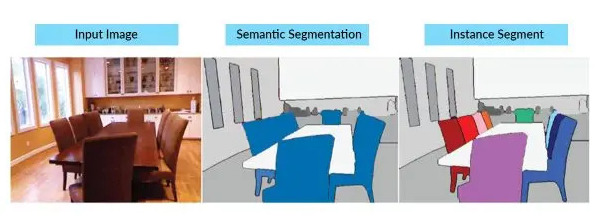
\includegraphics[scale=0.5]{segmentation}
  
\end{center}

\> De obicei, metodele de segmentare au in vedere urmatoarele cazuri:

\begin{itemize}

	\item discontinuitatea entitatilor observabile - in acest caz o metoda potrivita de segmentare ar fi detectia conturului
	\item similitudinea observabilelor - cele mai comune metode de segmentare folosite in acest caz sunt metoda regiunilor si metoda pragului

\end{itemize}

\newpage

\section{Detectarea contururilor}

\> Un contur poate fi reprezentat de o modificare brusca de lumina, culoare, umbra sau
textura din contextul unei imagini digitale. Analiza imaginilor folosind metode de
detectare a contururilor ajuta atat la solutionarea necesitatii de a extragere anumite obiecte
de interes din cadrul acestora cat si la filtrarea informatiei inutile.

\> Deoarece calitatea rezultatelor oferite de procesele de detectare poate fi afectata de cantitatea de zgomot prezenta in imagine,
un procedeu robust si bine stabilit de preprocesare si filtrare a acesteia este deseori necesar. 

\> Muchiile sunt modificări locale semnificative de intensitate într-o imagine digitală.
O muchie poate fi definită ca un set de pixeli conectați care formează o limită între două regiuni disjuncte.
Există trei tipuri de muchii: orizontale, verticale si diagonale.

\> Detectarea marginilor este o metodă de segmentare a unei imagini în regiuni de discontinuitate.
Este o tehnică utilizată pe scară largă în prelucrarea digitală a imaginilor, cum ar fi recunoasterea formelor ("pattern recognition") sau
extragerea caracteristicilor ("feature extraction").

\> Detectarea marginilor permite utilizatorilor să observe caracteristicile unei imagini pentru o schimbare semnificativă a nivelului de gri.
Această textură indică sfârșitul unei regiuni din imagine și începutul alteia.
Aceasta reduce cantitatea de date dintr-o imagine și păstrează proprietățile structurale ale imaginii. 

Operatorii de detectare a marginilor sunt de două tipuri: 

\begin{itemize}

  \item Gradient - operator bazat pe care calculează derivatele de ordinul întâi într-o imagine digitală,
  cum ar fi: operatorul Sobel, operatorul Prewitt, operatorul Robert
  \item Gaussian - operator bazat pe Gaussian care calculează derivatele de ordinul doi într-o imagine digitală,
  cum ar fi: detectorul de margini Canny, Laplacianul lui Gaussian

\end{itemize}

\begin{center}

  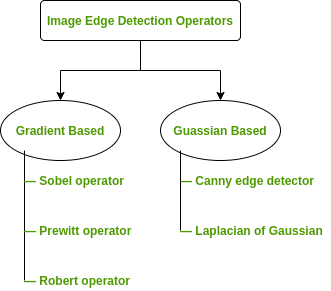
\includegraphics[scale=0.5]{operatori-detectare}
  
\end{center}

\newpage

\subsection{Operatorul Sobel}

\> Operatorul Sobel este un operator de diferențiere discretă.
Acesta calculează aproximarea gradientului funcției de intensitate a imaginii pentru detectarea marginilor imaginii.

\> Aplicat pe pixelii unei imagini, operatorul Sobel produce fie normala la un vector, fie vectorul gradient corespunzător.
Acesta Utilizează două nuclee sau măști 3 x 3 care sunt convolute cu imaginea de intrare pentru a calcula aproximările derivatei
verticale și, respectiv, orizontale. 

\begin{center}

  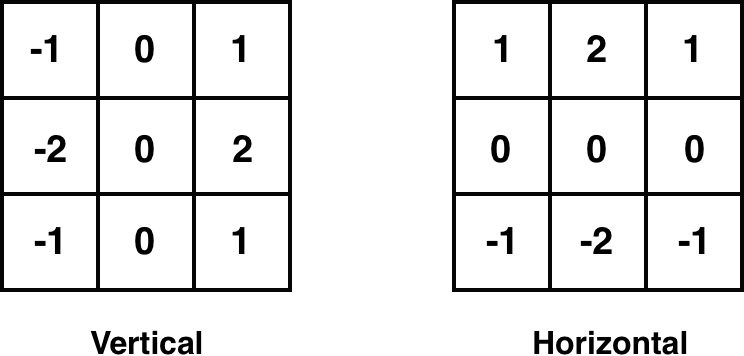
\includegraphics[scale=0.3]{sobel-mask.jpg}
  
\end{center}

\> Avantaje:
\begin{itemize}

  \item Calcul simplu și eficient în timp
  \item Foarte ușor la căutarea de margini netede

\end{itemize}

\> Limitari:
\begin{itemize}

  \item Punctele de direcție diagonală nu sunt păstrate întotdeauna
  \item Foarte sensibil la zgomot
  \item Nu este foarte precis în detectarea marginilor
  \item Detectarea cu margini groase și aspre nu dă rezultate corespunzătoare
  
\end{itemize}

\newpage

\subsection{Operatorul Prewitt}

\> Operatorul Prewitt este similar cu operatorul sobel. De asemenea, acesta detectează marginile verticale și orizontale ale unei imagini.
Este una dintre cele mai bune modalități de a detecta orientarea și magnitudinea unei imagini.
 
\begin{center}

  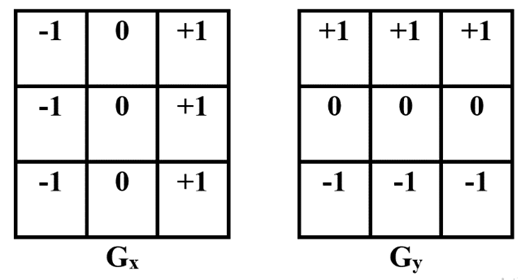
\includegraphics[scale=0.5]{prewitt}
  
\end{center}

\> Avantaje:
\begin{itemize}

  \item Performanță bună la detectarea marginilor verticale și orizontale
  \item Cel mai bun operator pentru a detecta orientarea unei imagini

\end{itemize}

\> Limitari:
\begin{itemize}

  \item Mărimea coeficientului este fixă și nu poate fi modificată
  \item Punctele de direcție diagonală nu sunt păstrate întotdeauna
  
\end{itemize}

\newpage


\subsection{Operatorul Robert}

\> Operatorul Robert calculează suma pătratelor diferențelor dintre pixelii adiacenți pe diagonală dintr-o imagine prin diferențiere discretă,
dupa care va face aproximarea gradientului.
\begin{center}

  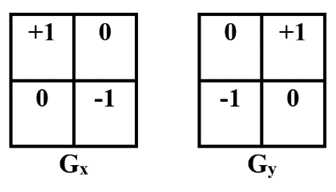
\includegraphics[scale=0.5]{robert}
  
\end{center}

\> Avantaje:
\begin{itemize}

  \item Detectarea marginilor și orientarea sunt foarte ușoare
  \item Punctele de direcție diagonală sunt păstrate

\end{itemize}

\> Limitari:
\begin{itemize}

  \item Foarte sensibil la zgomot
  \item Nu este foarte precis în detectarea marginilor
  
\end{itemize}

\newpage



\subsection{Operatorul Marr-Hildreth}

\> Operatorul Marr-Hildreth sau Laplacianul lui Gauss (LoG) este un operator bazat pe gaussian care utilizează Laplacianul
pentru a lua a doua derivată a unei imagini. Acesta funcționează foarte bine atunci când tranziția nivelului de gri pare a fi bruscă.

\> Funcționează pe baza metodei de trecere prin zero, adică atunci când derivata de ordinul doi trece prin zero, atunci acea locație specifică corespunde unui nivel maxim.
Aceasta se numește locație de margine. Aici, operatorul gaussian reduce zgomotul, iar operatorul laplacian detectează marginile ascuțite. 

\begin{center}

  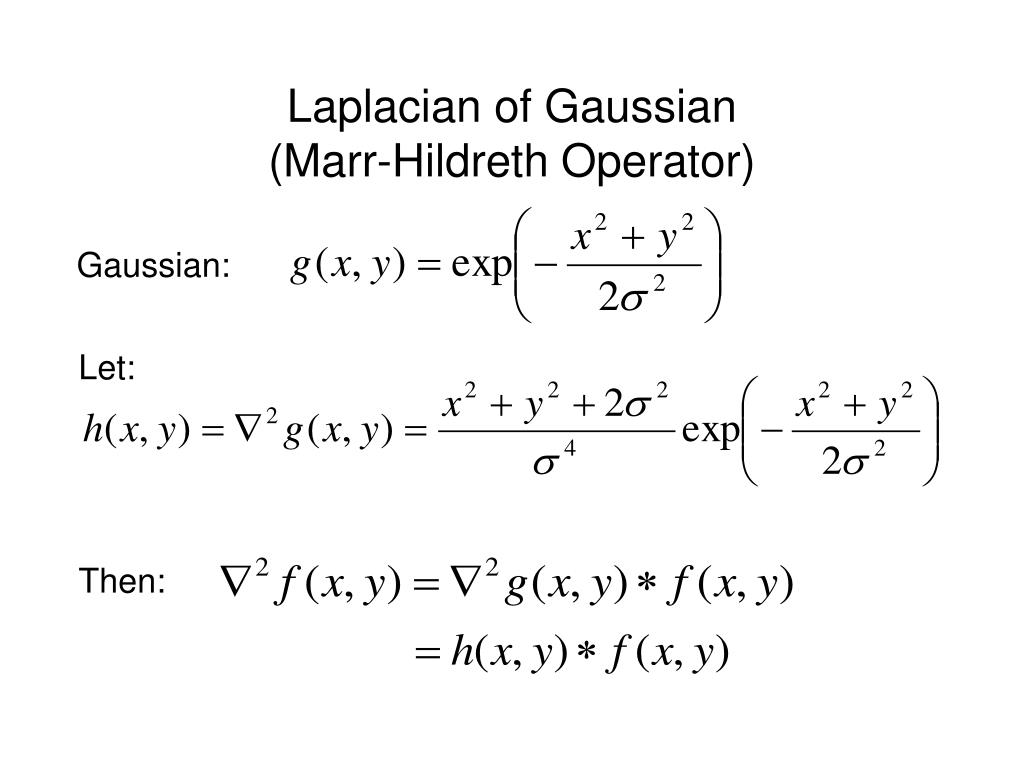
\includegraphics[scale=0.3]{marr-hildreth}
  
\end{center}

\> Avantaje:
\begin{itemize}

  \item Ușor de detectat marginile și diferitele orientări ale acestora
  \item Există caracteristici fixe în toate direcțiile
  
\end{itemize}

\> Limitari:
\begin{itemize}

  \item Foarte sensibil la zgomot
  \item Eroarea de localizare poate fi severă la marginile curbate
  \item Acesta generează răspunsuri zgomotoase care nu corespund unor muchii, așa-numitele "muchii false"
  
\end{itemize}

\newpage


\subsection{Operatorul Canny}

\> Operatorul Canny este un operator bazat pe gaussian pentru detectarea marginilor. 
Acest operator nu este sensibil la zgomot. Acesta extrage caracteristicile imaginii fără a afecta sau modifica caracteristicile.

\> Detectorul de margini Canny are un algoritm avansat derivat din munca anterioară a operatorului Marr-Hildreth.
Este o tehnică de detectare optimă a marginilor, utilizată pe scară largă. Acesta detectează marginile pe baza a trei criterii: 

\begin{itemize}

  \item Rata de eroare scăzută 
  \item Punctele de margine trebuie să fie localizate cu precizie 
  \item Ar trebui să existe doar un singur răspuns pe muchie

\end{itemize}

\begin{center}

  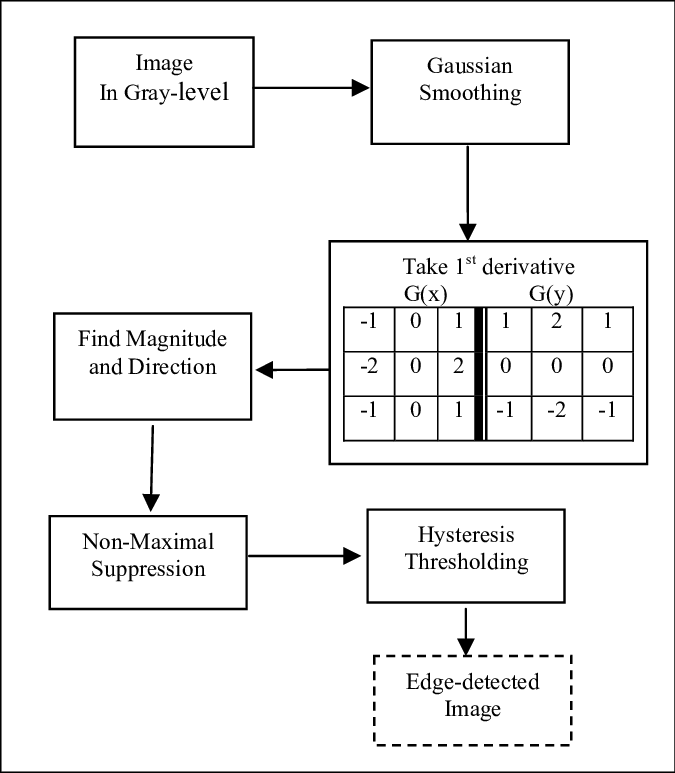
\includegraphics[scale=0.3]{canny}
  
\end{center}

\> Avantaje:
\begin{itemize}

  \item Are o localizare bună
  \item Acesta extrage caracteristicile imaginii fără a modifica caracteristicile
  \item Mai puțin sensibil la zgomot

\end{itemize}

\> Limitari:
\begin{itemize}

  \item Există o trecere falsă la zero
  \item Calcul complex și consumator de timp
  
\end{itemize}

\newpage

\section{Histograme de intensitate}

\subsection{Scurta descriere}

\> În contextul procesării imaginilor, histograma este folosita pentru reprezentarea distributiei valorilor intensității pixelilor.
Această reprezentare este un grafic care expune numărul de pixeli dintr-o imagine apartinand unei valori diferite de intensitate găsite în acea imagine.

\> Pentru o imagine în tonuri de gri pe 8 biți, există 256 de intensități diferite posibile, astfel încât histograma va afișa grafic 256 de numere
care descriu distribuția pixelilor între aceste valori ale tonurilor de gri. Histogramele pot fi, de asemenea, realizate pentru imaginile color -
fie se pot realiza histograme individuale fiecarui canal (in cazul spectrului RGB - roșu, verde și albastru), fie se poate realiza o histogramă tridimensională, 
în care cele trei axe reprezintă canalele roșu, albastru și verde, iar luminozitatea din fiecare punct reprezintă numărul de pixeli.
 
 \> Rezultatul exact al operațiunii depinde de implementare. Acesta poate fi pur și simplu o imagine a histogramei solicitate într-un format de
imagine adecvat sau poate fi un fișier de date care să reprezinte informatia incapsulata de histograma.


\begin{center}

  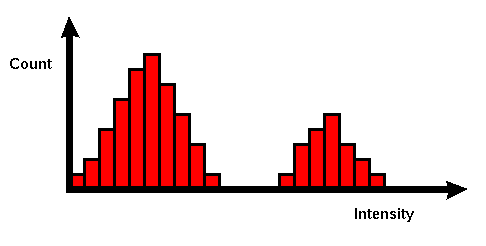
\includegraphics[scale=0.7]{histograma-intensitate}
  
\end{center}

\subsection{Cum functioneaza}

\> Procesul de aplicarea a acestei metode este foarte simplu:
imaginea este scanată într-o singură trecere (rand cu rand) și se va stoca o contorizare a numărului de pixeli găsiți pentru fiecare valoare de intensitate.
Aceasta contorizare este apoi utilizată pentru a construi o histogramă reprezentativa.

\newpage

\section{Exemplu de aplicatie}

\> Exemplul de aplicatie folosit pentru a demonstra cateva dintre tehnicile de preprocesare, recunoastere si clasificare
descrise anterior este reprezentat de un microserviciu scris in limbajul 'Go' al carui scop este extragerea textului digital din cadrul
unui document scanat.

\> De asemenea a fost realizata si o interfata pentru studiul si analiza eficientei microserviciului reprezentata de
o aplicatie web care pune la dispozitie o panza pe care putem desena diverse forme sau incarca imagini de pe disc si 
invoca functionalitati puse la dispozitie de microserviciul de recunoastere. 

\> Pentru mai multe detalii legate de implementari, acestea sunt puse la dispozitie pentru eventualii doritori (
\href{https://github.com/vlad-a-barbu/gocr}{github.com/vlad-a-barbu/gocr} si \href{https://github.com/vlad-a-barbu/gocr-ui}{github.com/vlad-a-barbu/gocr-ui}).

\> Structura si modul de functionare al microserviciului este descris de urmatorii pasi:

\begin{itemize}

  \item Preprocesarea documentului 
  \item Extragerea obiectelor de interes (subimagini reprezentand caracterele ce urmeaza a fi identificate) 
  \item Pentru fiecare candidat al procesului de recunoastere se vor genera cate doua histograme reprezentand
  distributia pixelilor de interes atat din perspectiva verticala cat si din perspectiva orizontala
  \item Pentru fiecare candidat al procesului de recunoastere se va genera o pereche de expresii regulate
  reprezentand numarul de intervale continue de pixeli de interes continuti pe randurile deprinse din perspectiva verticala,
  respectiva din perspectiva orizontala
  \item Microserviciul se va folosi de un set de histograme si perechi de expresii de referinta in baza carora se va face clasificarea
  
\end{itemize}

\> * Setul de date de referinta este rezultat din incarcarea unei imagini de baza care va contine cate o subimagine reprezentativa
fiecarui caracter folosit in documentele ce urmeaza sa fie analizate - spre exemplu imaginea de baza ar putea fi reprezentata de
alfabetul limbajului in care au fost scrise documentele ce urmeaza a fi identificate. Pentru simplitate se pot folosi reprezentari ale alfabetului englez
in diverse fonturi des intalnite: helvetica, arial, times new roman, etc.

\> * Scopul microserviciului nu este acela de a oferi consumatorilor sai o metoda robusta si generala de identificare si clasificare. Acesta serveste
drept aplicatie demonstrativa, suport de invatare si experimentare pentru diverse metode de procesare a imaginilor digitale.

\newpage

\subsection{Metode de preprocesare}

Imagine folosita de-a lungul procesului de recunoastere:

\begin{center}

  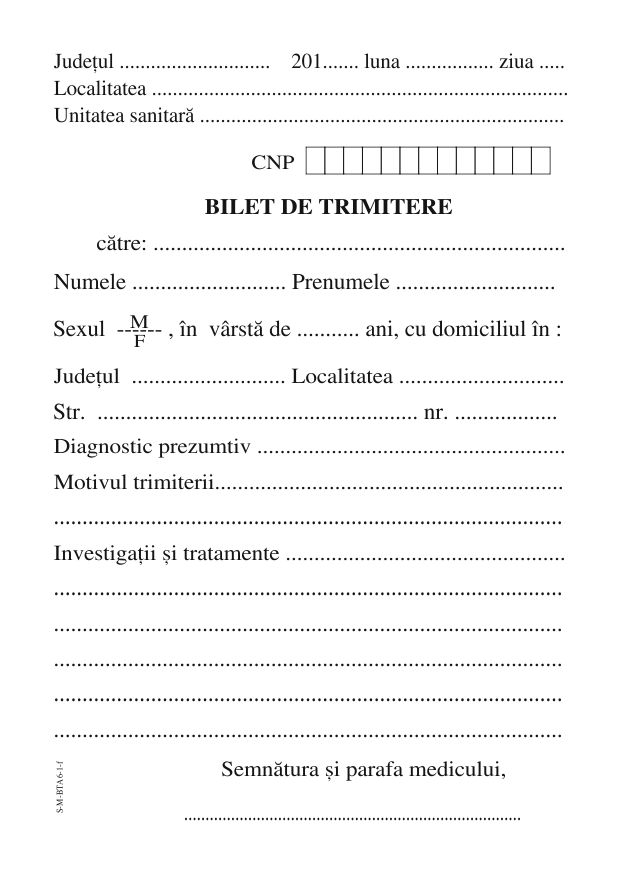
\includegraphics[scale=0.7]{imagine-analizata.jpg}
  
\end{center}

\> Putem observa efectele conversiei la imagine tip Grayscale - a fost realizata maparea din spectrul de culori RGB in spectrul Grayscale
(tonuri de gri) folosind urmatoarea formula de calcul a luminantei relative:

\begin{center}

  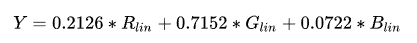
\includegraphics[scale=1]{formula-luminanta}
  
\end{center}


\begin{center}

  
\includegraphics[scale=0.5]{efecte-grayscale}
  
\end{center}

\newpage

\> Efectele aplicarii unui filtru tip threshold alegand o valoare maxima acceptata pentru luminanta pixelilor 
(se observa fenomenul de fragmentare a caracterelor):

\begin{center}

  
\includegraphics[scale=1]{fragmentare}
  
\end{center}

\> Efectele aplicarii unei masti de interpolare pe verticala si orizontala a pixelilor vecini pentru a rezolva problema fragmentarii:

\begin{center}

  
\includegraphics[scale=0.5]{lipire-normala}
  
\end{center}

\> Efectele aplicarii unei masti de interpolare pe verticala, orizontala si diagonala a pixelilor vecini pentru a rezolva problema fragmentarii
(metoda mai agresiva, se poate observa fenomenul de "lipire" a entitatilor observabile):

\begin{center}

  
\includegraphics[scale=1]{lipire-agresiva}
  
\end{center}

\> Selectarea obiectelor de interes a fost realizata prin procesul de parcurgere a imaginii preprocesate rand cu rand,
si aplicarea metodelor de segmentare descrise anterior pentru a grupa pixelii de interes in mai multe clase de entitati observabile.

\> Pentru implementare s-au folosit algoritmi de tip 'Fill' la momentul interceptarii unui pixel de interes, luand in considerare atat
vecinii de pe orizontala si verticala cat si vecinii de pe diagonala (proces eficientizat de mastile si filtrele descrise mai sus).

\newpage

\subsection{Formarea descriptorilor de referinta}

\> Urmatoarea imagine prezinta alfabetul englez de caractere reprezentata de fontul Helvetica (unul dintre cele mai populare 
fonturi pentru documentele digitale):

\begin{center}

  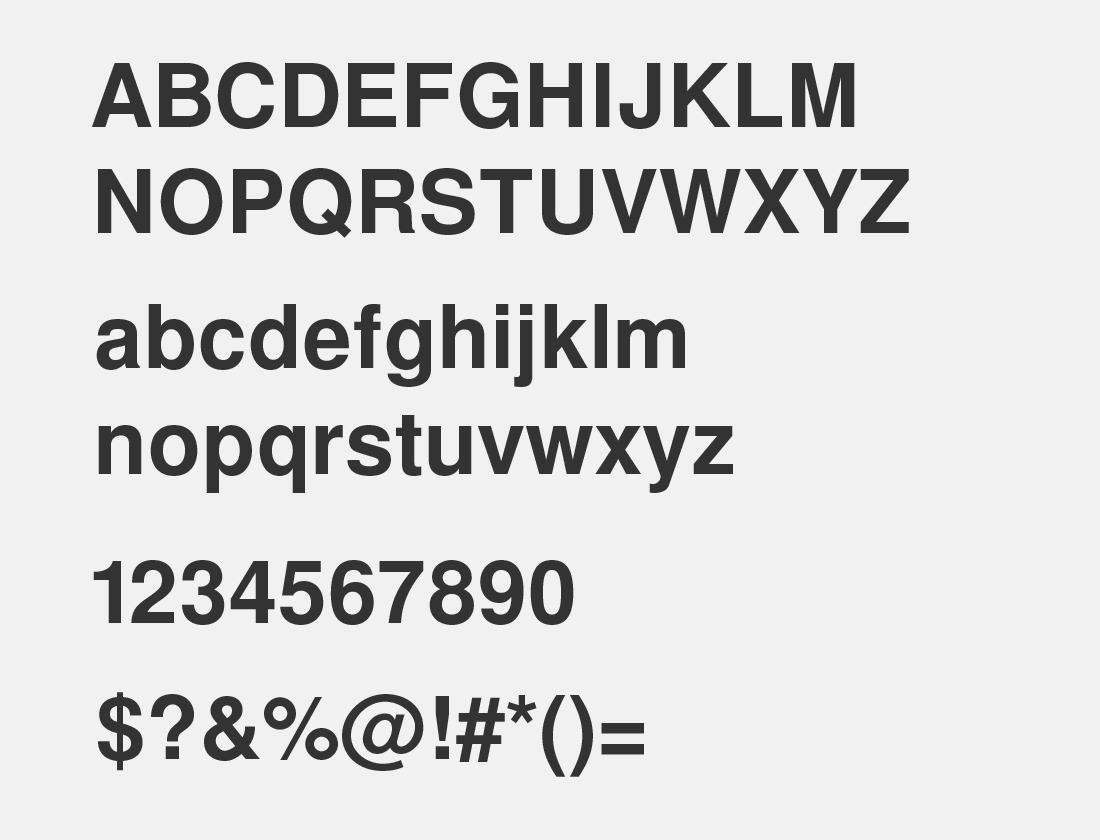
\includegraphics[scale=0.1]{helvetica}
  
\end{center}

\> In baza acestei imagini s-a extras pe rand fiecare caracter, si i-au fost asociate urmatoarele metadate:

\begin{itemize}

  \item O pereche de expresii regulate reprezentand frecventele pixelilor de interes pe randuri si pe coloane
  \item O histograma urmarind distributia pixelilor de interes din perspectiva orizontala
  \item O histograma urmarind distributia pixelilor de interes din perspectiva verticala
  
\end{itemize}

\> Histogramele vor fi folosite drept factori cantitativi in procesul de clasificare,
urmand ca expresiile sa intervina drept factor calitativ (descriptori de 'forma' pentru caracterele analizate).
  
\> Exemple de expresii regulate de referinta:

\begin{center}

  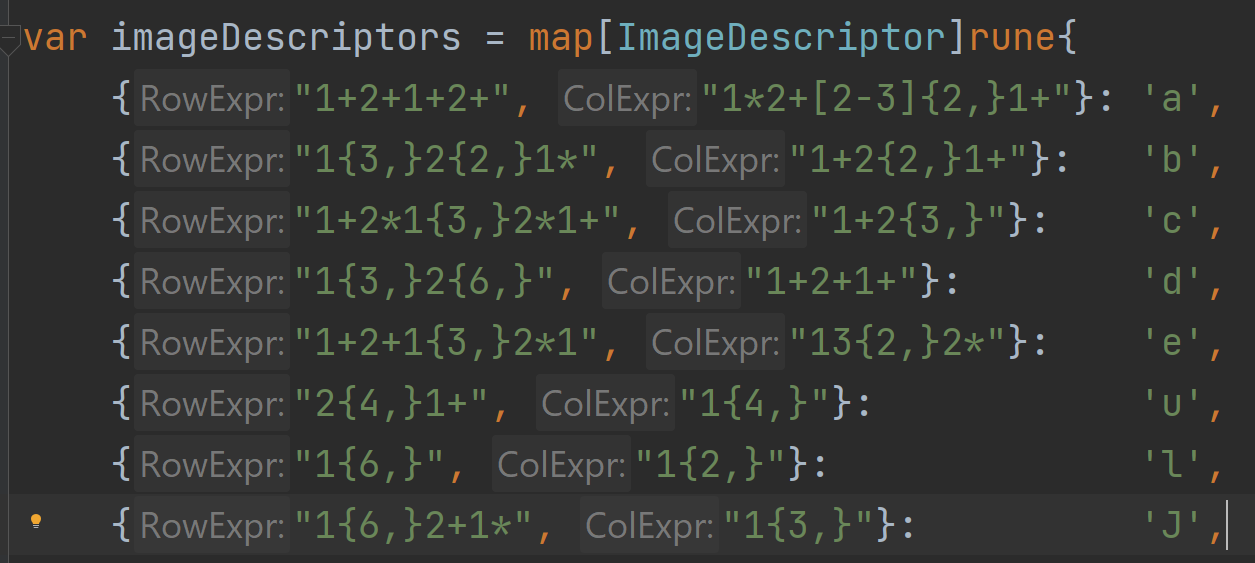
\includegraphics[scale=0.6]{model-expresii}
  
\end{center}
  
\newpage

\subsection{Generarea histogramelor}

\> Subimagine a caracterului de referinta analizat:

\begin{center}

  
\includegraphics[scale=1]{hist-image}
  
\end{center}

\> Histograma urmarind distributia pixelilor de interes din perspectiva orizontala (frecventa acestora pe randuri):

\begin{center}

  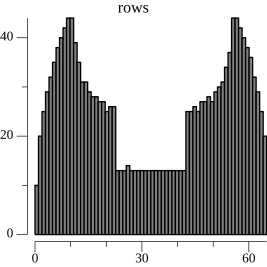
\includegraphics[scale=0.5]{hist-rows}
  
\end{center}

\> Histograma urmarind distributia pixelilor de interes din perspectiva verticala (frecventa acestora pe coloane):

\begin{center}

  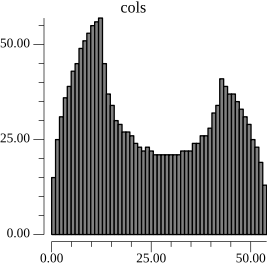
\includegraphics[scale=0.5]{hist-cols}
  
\end{center}

\newpage

\begin{thebibliography}{widest entry}
  \bibitem[1]{key1} \href{https://en.wikipedia.org/wiki/Image_noise}{en.wikipedia.org/wiki/ImageNoise}
  \bibitem[2]{key2} \href{https://www.analytixlabs.co.in/blog/what-is-image-segmentation/}{analytixlabs.co.in/blog/what-is-image-segmentation/}
  \bibitem[3]{key3} \href{https://medium.com/@shashikadilhani97/digital-image-processing-filters-832ec6d18a73}{medium.com/@shashikadilhani97/digital-image-processing-filters}
  \bibitem[4]{key4} \href{https://www.geeksforgeeks.org/image-edge-detection-operators-in-digital-image-processing/}{geeksforgeeks.org/image-edge-detection-operators-in-digital-image-processing/}
  \bibitem[5]{key5} \href{http://old.upm.ro/facultati_departamente/stiinte_litere/conferinte/situl_integrare_europeana/Lucrari2/Ioan_Ispas.pdf}{old.upm.ro/facultati-departamente/stiinte-litere/conferinte/situl-integrare-europeana/Lucrari2/Ioan-Ispas.pdf}
  \bibitem[6]{key6} \href{http://www.perform.usv.ro/rapoarte/10/raport_cercetare_1.pdf}{perform.usv.ro/rapoarte/10/raport-cercetare-1.pdf}
  \bibitem[7]{key7} \href{https://rria.ici.ro/wp-content/uploads/2020/10/Complex_Architectures_Used_in_Image_Parallel_Processing.pdf}{rria.ici.ro/wp-content/uploads/2020/10/Complex-Architectures-Used-in-Image-Parallel-Processing.pdf}
  \bibitem[8]{key8} \href{https://www.miv.ro/books/MIvanovici_PI.pdf}{www.miv.ro/books/MIvanovici-PI.pdf}
  \bibitem[9]{key9} \href{https://www.researchgate.net/profile/Gaurav-Gupta-53/publication/325681876_Image_Filtering_Algorithms_and_Techniques_A_Review/links/5b1e1ab0aca272021cf585c9/Image-Filtering-Algorithms-and-Techniques-A-Review.pdf}{researchgate.net/profile/Gaurav-Gupta-53/publication/Image-Filtering-Algorithms-and-Techniques-A-Review.pdf}
  \bibitem[10]{key10} \href{https://books.google.ro/books?id=xeWpCAAAQBAJ&printsec=frontcover&redir_esc=y#v=onepage&q&f=false}{books.google.ro/Theo-Pavlidis-Algorithms-for-Graphics-and-Image-Processing}
  \bibitem[11]{key11} \href{https://homepages.inf.ed.ac.uk/rbf/HIPR2/histgram.htm}{homepages.inf.ed.ac.uk/rbf/HIPR2/histgram}
\end{thebibliography} 

\end{document}
